\ifdefined\niveldos\else
\documentclass[12pt,letterpaper]{report}
 
%Russian-specific packages
%--------------------------------------
\usepackage[T2A]{fontenc}
\usepackage[utf8]{inputenc}
\usepackage[russian]{babel}
\usepackage[mathscr]{euscript}
\usepackage{amsmath,amsthm,amssymb,latexsym,amsfonts}
\usepackage{pythonhighlight}
\usepackage{lipsum}
\usepackage{soul}
\usepackage{amsmath,amssymb}
\usepackage{parskip}
\usepackage{graphicx}
\usepackage{mathtools}
\usepackage[usestackEOL]{stackengine} 
\usepackage{tocloft}
\usepackage{xcolor}
\usepackage{hyperref}
\usepackage{tikz}
\usepackage{thmtools}
\usepackage{amsthm}
\usepackage{mathtools}
\usepackage{pdfcomment}
\usepackage{blindtext}
\usepackage{todonotes}
\usepackage{import}
\usepackage{hyphsubst}
\usepackage{bookmark}

\graphicspath{ {./images/} }
%%

\DeclarePairedDelimiter\abs{\lvert}{\rvert}%
\DeclarePairedDelimiter\norm{\lVert}{\rVert}%

% Swap the definition of \abs* and \norm*, so that \abs
% and \norm resizes the size of the brackets, and the 
% starred version does not.
\makeatletter
\let\oldabs\abs
\def\abs{\@ifstar{\oldabs}{\oldabs*}}
%
\let\oldnorm\norm
\def\norm{\@ifstar{\oldnorm}{\oldnorm*}}
\makeatother

\newtheorem{theorem}{Предложение}
\newtheorem*{theorem-non}{Предложение}
\newtheorem*{lemma}{Лемма}
\theoremstyle{definition}
\newtheorem*{conj}{Определение}
\declaretheorem[numbered=no]{definition}

% Definindo novas cores
\definecolor{verde}{rgb}{0.25,0.5,0.35}
\definecolor{jpurple}{rgb}{0.5,0,0.35}
\definecolor{darkgreen}{rgb}{0.0, 0.2, 0.13}
%\definecolor{oldmauve}{rgb}{0.4, 0.19, 0.28}
% Configurando layout para mostrar codigos Java
\usepackage{listings}

\newcommand{\estiloJava}{
\lstset{
    language=Java,
    basicstyle=\ttfamily\small,
    keywordstyle=\color{jpurple}\bfseries,
    stringstyle=\color{red},
    commentstyle=\color{verde},
    morecomment=[s][\color{blue}]{/**}{*/},
    extendedchars=true,
    showspaces=false,
    showstringspaces=false,
    numbers=left,
    numberstyle=\tiny,
    breaklines=true,
    backgroundcolor=\color{cyan!10},
    breakautoindent=true,
    captionpos=b,
    xleftmargin=0pt,
    tabsize=2
}}

\newcommand{\estiloR}{
  \lstset{ %
    language=R,                     % the language of the code
    basicstyle=\footnotesize,       % the size of the fonts that are used for the code
    numbers=left,                   % where to put the line-numbers
    numberstyle=\tiny\color{gray},  % the style that is used for the line-numbers
    stepnumber=1,                   % the step between two line-numbers. If it's 1, each line
                                    % will be numbered
    numbersep=5pt,                  % how far the line-numbers are from the code
    backgroundcolor=\color{white},  % choose the background color. You must add \usepackage{color}
    showspaces=false,               % show spaces adding particular underscores
    showstringspaces=false,         % underline spaces within strings
    showtabs=false,                 % show tabs within strings adding particular underscores
    frame=single,                   % adds a frame around the code
    rulecolor=\color{black},        % if not set, the frame-color may be changed on line-breaks within not-black text (e.g. commens (green here))
    tabsize=2,                      % sets default tabsize to 2 spaces
    captionpos=b,                   % sets the caption-position to bottom
    breaklines=true,                % sets automatic line breaking
    breakatwhitespace=false,        % sets if automatic breaks should only happen at whitespace
    title=\lstname,                 % show the filename of files included with \lstinputlisting;
                                    % also try caption instead of title
    keywordstyle=\color{blue},      % keyword style
    commentstyle=\color{darkgreen},   % comment style
    stringstyle=\color{red},      % string literal style
    escapeinside={\%*}{*)},         % if you want to add a comment within your code
    morekeywords={*,...}          % if you want to add more keywords to the set
}}

\newcommand{\Z}{\mathbb{Z}}
\newcommand{\Q}{\mathbb{Q}}
\newcommand{\N}{\mathbb{N}}
\newcommand{\R}{\mathbb{R}}
\newcommand{\follow}{\textbf{\textit{Следствие:}}}
\newcommand{\notice}{\underline{\textit{Замечание }}}

\newcommand*\circled[1]{\tikz[baseline=(char.base)]{
            \node[shape=circle,draw,inner sep=2pt] (char) {#1};}}

\definecolor{linkcolor}{HTML}{47528f} % цвет ссылок
\definecolor{urlcolor}{HTML}{47528f} % цвет гиперссылок
\hypersetup{pdfstartview=FitH,  linkcolor=linkcolor,urlcolor=urlcolor, colorlinks=true}
\newcommand{\RomanNumeralCaps}[1]
  {\MakeUppercase{\romannumeral #1}}
\usepackage{titlesec}
\renewcommand{\thesection}{\arabic{section}}
\renewcommand{\listtheoremname}{Определения и теоремы}
\renewcommand\qedsymbol{$\blacksquare$}
\newcommand\oast{\stackMath\mathbin{\stackinset{c}{0ex}{c}{0ex}{\ast}{\bigcirc}}}
\makeatletter
\renewenvironment{proof}[1][\proofname]{%
   \par\pushQED{\qed}\normalfont%
   \topsep6\p@\@plus6\p@\relax
   \trivlist\item[\hskip\labelsep\bfseries#1\@addpunct{.}]%
   \ignorespaces
}{%
   \popQED\endtrivlist\@endpefalse
}
\makeatother
%--------------------------------------
\DeclareMathOperator{\Mr}{M_{\mathbb{R}}}
\addtolength{\oddsidemargin}{-.875in}
	\addtolength{\evensidemargin}{-.875in}
	\addtolength{\textwidth}{1.75in}

	\addtolength{\topmargin}{-.875in}
    \addtolength{\textheight}{1.75in}
%--------------------------------------
\def\calloutsym{%
  \ensurestackMath{%
  \scalebox{1.7}{\color{red}\stackunder[0pt]{\bigcirc}{\downarrow}}}%
}
\def\calloutsymup{%
  \ensurestackMath{%
  \scalebox{1.7}{\color{red}\stackon[0pt]{\bigcirc}{\uparrow}}}%
}
\newcommand\callouttext[1]{%
  \def\stacktype{S}\renewcommand\useanchorwidth{T}\stackText%
  \stackunder{\calloutsym}{\scriptsize\Longstack{#1}}\stackMath%
}
\newcommand\callout[3][2.5pt]{%
  \def\stacktype{L}\stackMath\stackunder[#1]{#2}{\callouttext{#3}}%
}
\newcommand\callouttextup[1]{%
  \def\stacktype{S}\renewcommand\useanchorwidth{T}\stackText%
  \stackon{\calloutsymup}{\scriptsize\Longstack{#1}}\stackMath%
}
\newcommand\calloutup[3][1.5pt]{%
  \def\stacktype{L}\stackMath\stackunder[#1]{#2}{\callouttextup{#3}}%
}
\begin{document}

\clearpage
%% temporary titles
% command to provide stretchy vertical space in proportion
\newcommand\nbvspace[1][3]{\vspace*{\stretch{#1}}}
% allow some slack to avoid under/overfull boxes
\newcommand\nbstretchyspace{\spaceskip0.5em plus 0.25em minus 0.25em}
% To improve spacing on titlepages
\newcommand{\nbtitlestretch}{\spaceskip0.6em}
\pagestyle{empty}
\begin{center}
\bfseries
\nbvspace[1]
\Huge
{\nbtitlestretch\huge
КОНСПЕКТ ЛЕКЦИЙ ПО ЛИНЕЙНОЙ АЛГЕБРЕ}

\nbvspace[1]
\normalsize

СПбГУ, МКН, СП, 1 курс\\
ЛЕКТОР: ЖУКОВ ИГОРЬ БОРИСОВИЧ
\nbvspace[1]
\\
\Large СОСТАВИТЕЛИ:\\[0.5em]
\footnotesize 
Андрей \href{https://github.com/K-dizzled}{K-dizzled} Козырев, 
Никита  \href{https://github.com/muldrik}{muldrik} Митцев,
Максим \href{https://github.com/maxmartynov08}{maxmartynov08} Мартынов,\\ 
Семён \href{https://github.com/SmnTin}{SmnTin} Паненков,
Марк \href{https://github.com/markprudnikov}{markprudnikov} Прудников,
Арсений \href{https://github.com/ElectFreak}{ElectFreak} Юсуфов

\nbvspace[2]

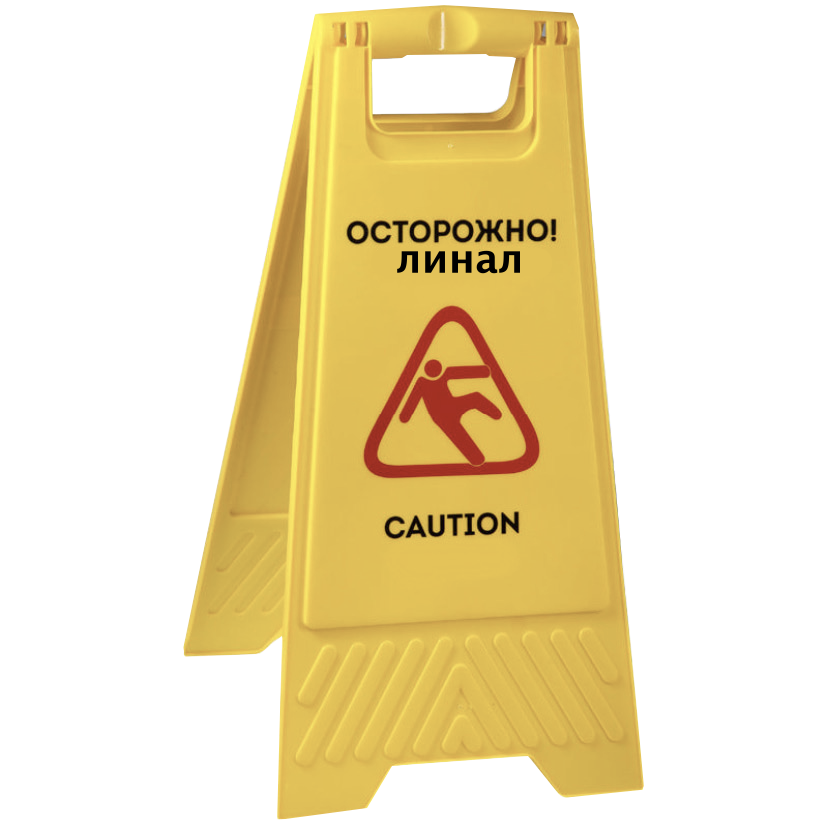
\includegraphics[width=4.0in]{./images/DangerLinal2.png}
\nbvspace[3]
\normalsize

\large
ЗИМА 2020
\nbvspace[1]
\end{center}
\newpage
\pagestyle{plain}
\fi
%\maketitle
%%%%%%%%%%%%%%%%%%%%%%%%%%%%%%%%%%
%                                %
%                                %
%        Table of content        %
%                                %
%                                %
%%%%%%%%%%%%%%%%%%%%%%%%%%%%%%%%%%
\tableofcontents
%\listoftheorem-nons[ignore={lemma},show={conj, theorem-non}]
% To show Table of contents with
% definitions and lemmas
%----------------------------------------
% \listoftheorem-nons[ignoreall,show={lemma}]
% \listoftheorem-nons[ignoreall,show={conj}]
\newpage
\begin{normalsize}
\chapter*{Первый семестр. Первая четверть}
\import{sections/}{ticket01.tex}
$ $
\import{sections/}{ticket02.tex}
$ $
\import{sections/}{ticket03.tex}
$ $
\import{sections/}{ticket04.tex}
$ $
\import{sections/}{ticket05.tex}
$ $
\import{sections/}{ticket06.tex}
$ $
\import{sections/}{ticket07.tex}
$ $
\import{sections/}{ticket08.tex}
$ $
\import{sections/}{ticket09.tex}
$ $
\import{sections/}{ticket10.tex}
$ $
\import{sections/}{ticket11.tex}
$ $
\import{sections/}{ticket12.tex}
$ $
\import{sections/}{ticket13.tex}
$ $
\import{sections/}{ticket14.tex}
$ $
\import{sections/}{ticket15.tex}
$ $
\import{sections/}{ticket16.tex}
$ $
\import{sections/}{ticket17.tex}
$ $
\import{sections/}{ticket18.tex}
$ $
\import{sections/}{ticket19.tex}
$ $
\import{sections/}{ticket20.tex}
$ $
\import{sections/}{ticket21.tex}
$ $
\import{sections/}{ticket22.tex}
$ $
\import{sections/}{ticket23.tex}
$ $
\import{sections/}{ticket24.tex}
$ $
\import{sections/}{ticket25.tex}
$ $
\import{sections/}{ticket26.tex}
$ $
\import{sections/}{ticket27.tex}
$ $
\import{sections/}{ticket28.tex}
$ $
\import{sections/}{ticket29.tex}
$ $
\import{sections/}{ticket30.tex}
$ $
\import{sections/}{ticket31.tex}
$ $
\import{sections/}{ticket32.tex}
$ $
\import{sections/}{ticket33.tex}
$ $
\import{sections/}{ticket34.tex}
$ $
\import{sections/}{ticket35.tex}
$ $
\import{sections/}{ticket36.tex}
$ $
\import{sections/}{ticket37.tex}
$ $
\import{sections/}{ticket38.tex}
$ $
\import{sections/}{ticket39.tex}
$ $
\import{sections/}{ticket40.tex}
$ $
\import{sections/}{ticket41.tex}
$ $
\import{sections/}{ticket42.tex}
$ $
\import{sections/}{ticket43.tex}
$ $
\import{sections/}{ticket44.tex}
$ $
\end{normalsize}
\end{document} 